\documentclass[conference]{IEEEtran}
\usepackage[utf8]{inputenc}
\usepackage{amsmath}
\usepackage{amssymb}
\usepackage{tikz}
\usetikzlibrary{arrows,shapes,chains,matrix,positioning,scopes,patterns,calc,
decorations.markings,
decorations.pathmorphing,
}
\usepackage{pgfplots}
\pgfplotsset{compat=1.3}
\usepgflibrary{shapes}

\newcommand{\wv}{\ensuremath{\mathbf{w}}}

\newcommand{\Am}{\ensuremath{\mathbf{A}}}

\newcommand{\vv}{\ensuremath{\mathbf{v}}}

\newcommand{\sv}{\ensuremath{\mathbf{s}}}

\newcommand{\xv}{\ensuremath{\mathbf{x}}}

\newcommand{\ev}{\ensuremath{\mathbf{e}}}

\begin{document}

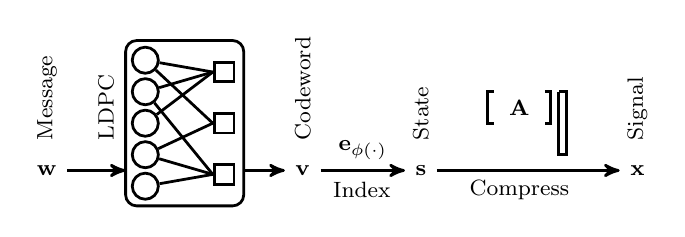
\begin{tikzpicture}
  [
  font=\footnotesize, >=stealth', line width=1pt,
  check/.style={rectangle, minimum height=2.5mm, minimum width=2.5mm, draw=black},
  varnode/.style={circle, minimum size=2mm, draw=black},
  mmse/.style={rectangle, minimum height=7.5mm, minimum width=25mm, rounded corners, draw=black},
  quantity/.style={rectangle, minimum height=8mm, minimum width=8mm, rounded corners, draw=black},
  multiply/.style={trapezium, trapezium angle=75, draw=black, minimum width=10mm, minimum height=8mm, rounded corners}
  ]



\node[rotate=90,anchor=west] (message) at (-0.25,0.25) {Message};
\node (bits) at (-0.25,0) {$\wv$};

\node[rotate=90,anchor=west] (ldpc) at (0.5,0.25) {LDPC};
\draw[draw=black, rounded corners] (0.75, -0.45) rectangle (2.25,1.65);
\foreach \s in {1,2,3,4,5} {
  \node[varnode] (var-\s) at (1,0.4*\s-0.6) {};
}
\foreach \c in {1,2,3} {
  \node[check] (check-\c) at (2,0.65*\c-0.7) {};
}
\draw (var-5) -- (check-3.west);
\draw (var-4) -- (check-3.west);
\draw (var-3) -- (check-3.west);
\draw (var-2) -- (check-2.west);
\draw (var-5) -- (check-2.west);
\draw (var-4) -- (check-1.west);
\draw (var-2) -- (check-1.west);
\draw (var-1) -- (check-1.west);

\foreach \v in {5.75} {
  \draw[line width=1pt] (\v-0.325,1) -- (\v-0.4,1) -- (\v-0.4,0.6) -- (\v-0.325,0.6);
  \draw[line width=1pt] (\v+0.325,1) -- (\v+0.4,1) -- (\v+0.4,0.6) -- (\v+0.325,0.6);
  \draw[line width=1pt] (\v+0.5,1) -- (\v+0.5,0.2) -- (\v+0.6,0.2) -- (\v+0.6,1) -- (\v+0.5,1);
  \node at (\v,0.8) {$\Am$};
}

\node[rotate=90,anchor=west] (codeword) at (3,0.25) {Codeword};
\node (symbols) at (3,0) {$\vv$};

\node (indexing) at (3.75,-0.25) {Index};

\node[rotate=90,anchor=west] (state) at (4.5,0.25) {State};
\node (index) at (4.5,0) {$\sv$};

\node (compression) at (5.75,-0.25) {Compress};

\node[rotate=90,anchor=west] (signal) at (7.25,0.25) {Signal};
\node (x) at (7.25,0) {$\xv$};

\draw[->] (bits) to (0.75,0);
\draw[->] (2.25,0) to (symbols);
\draw[->] (symbols) to node[above]{$\ev_{\phi(\cdot)}$} (index);
\draw[->] (index) to (x);

\end{tikzpicture}

\end{document}